\documentclass[11pt]{article}
\usepackage[top=20mm,bottom=30mm,left=20mm,right=20mm]{geometry}
\usepackage[utf8]{inputenc}
\usepackage{parskip}
\usepackage{abstract}

% Mathy stuff
\usepackage{physics}
\usepackage{siunitx}
\usepackage{amsmath}
\usepackage[version=4]{mhchem}

% Visual stuff
\usepackage{graphics}
\usepackage{tikz}
\usetikzlibrary{math}
\usepackage{stackengine}
\usepackage{float}

% Misc
\usepackage{hyperref}
\usepackage{cleveref}
\usepackage{lipsum}

\renewcommand{\abstractname}{}    % clear the title
\renewcommand{\absnamepos}{empty} % originally center

\setlength{\parskip}{2ex}
\setlength{\parindent}{0em}

\begin{document}
\pagenumbering{gobble}
\begin{center}
	\LARGE
	\textbf{Molecular Automata} \\
	\vspace{0.3em}
	\normalsize
	\textit{Jan Kocka, Jaime Agudo-Canalejo, Kabir Husain} \\
	\vspace{1em}
\end{center}

\begin{abstract}
	% Background
	% Cells must somehow store information/have memory and make decisions... \\
	Cells store and process information, largely through regulatory networks etc. but overall this is not understood at the level of information processing.
	Considerable effort is also being put into devising synthetic biological systems which can process information, a field known as molecular computation.
	Both fields are focused on DNA being the memory which stores information with molecular machines operating on it.
	However, this is not necessarily the case, we look at the information storage capability of an out-of-equilibrium allosteric complex.
	% What we/the model
	Here we build a thermodynamically consistent kinetic model of a molecular complex made of identical subunits each in one of two states (e.g., structural conformations, phosphorylation).
	We then analyse the dynamics of the complex as we allow each subunit's state to be changed by driven enzymes which act conditionally based on the states of the subunit's neighbours.
    We identify a set of simplest such systems and identify a one-to-one mapping between those and elementary cellular automata rules.
    % We identify and use a one-to-one mapping between each of a set of minimal such systems to an elementary cellular automata rule.

    Want to get accross: we look at the simplest/minimal systems of which there are a discrete count of, we find a one-to-one mapping to ECA rule (which we use to identify symmetries)

	We identify a rich set of behaviours including multi-stability and dynamical steady states in various geometries.
    We further draw an analoogy of each of the 256 possible minimal rules to a corresponding cellular automata rule and highlight the difference.
	% We identify a one to one map between such systems and elementary cellular automata rules and point out the differences.

	% We study the behaviour of a complex made of identical subunits, each in one of two states (e.g., structural conformations, phosphorylation).
	% We build a thermodynamically consistent kinetic model where the rate of changing the state of any one monomer can depend on the states of its neighbours.

	% Results/what we find from the model
	% We identify a connection between any such system and a cellular automata rule

	% Here we study the behaviour of a molecular complex made of identical subunits capable of changing between two states (e.g., structural conformations).
	% Here we study the behaviour of a molecular complex made of identical subunits, each allowed to change between two states, under the

	% Results/promises

	% % General introduction to topology in biology/biophysics - 98 words
	% Despite noisiness in the cellular environment, molecular systems show a high degree of robustness.
	% A recent new direction in understanding this apparent paradox is the study of topologically protected states in stochastic systems, which robustly confine the dynamics of the system to a lower-dimensional space.
	% However, it is unclear what the minimal biochemical ingredients are for such states to occur.
	%
	% % Getting into the project - ~110 words
	% Here, we study topological features in a non-equilibrium, thermodynamically-consistent model of a molecular assembly, made of subunits that undergo futile cycles of conformational change and phosphorylation.
	% When the subunits interact allosterically with each other, we find global, concerted cycles that emerge at the scale of the whole assembly.
	% These involve only a small subset of all possible conformations, analogous to topological edge currents in quantum systems.
	% We map out the kinetics, energetics, and biochemical interactions necessary to obtain distinct classes of topological behaviour.
	%
	% % Results-ish ->
	% Our results suggest that topological states can provide a minimal description of molecular coordination in protein complexes, such as circadian oscillators (e.g. KaiABC) or polymer assembly and disassembly (e.g. microtubules).
	% More broadly, our results demonstrate that stereotyped dynamics can arise purely from non-equilibrium kinetic effects, without the need for an underlying energy landscape to channel them.
\end{abstract}

% \vfill
% \begin{figure}[H]
% 	\centering
% 	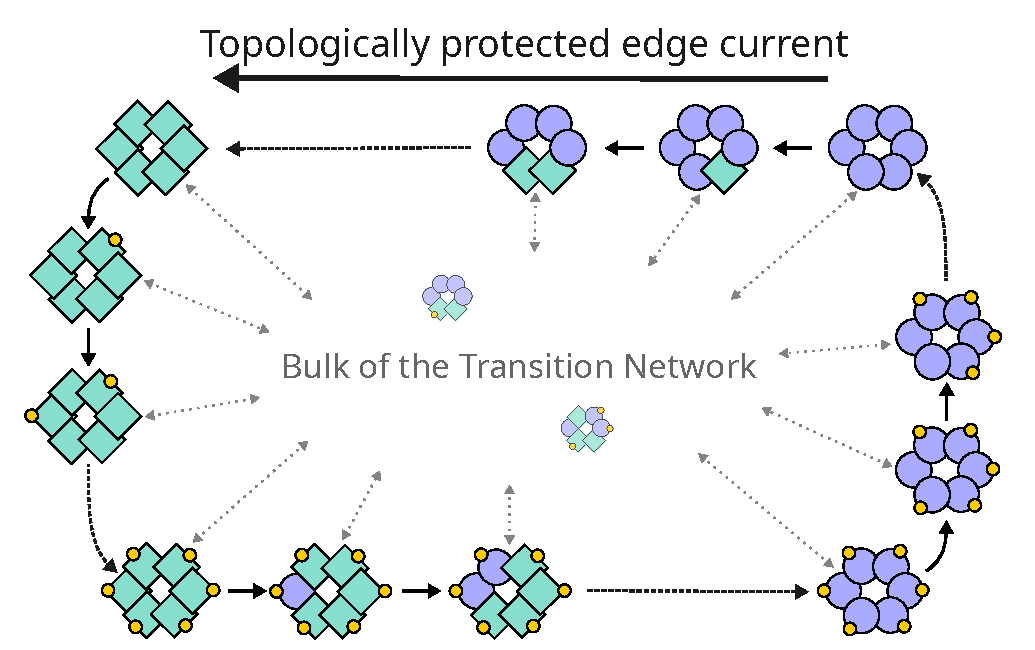
\includegraphics[width=\textwidth]{diagram/diagram_circly2.pdf}
% \end{figure}

\newpage

\newpage
\section{New Notes}
\begin{itemize}
	\item describe the model
	      \begin{itemize}
		      \item Identical subunits
		      \item Out-of-equilibrium + kinetic model
		      \item Rates depend on nearest neighbors
		      \item Thermodynamically consistent, but maximally driven
	      \end{itemize}
	\item what we find
	      \begin{itemize}
		      \item connection to cellular automata (classic model of computation)
		      \item rich set of behaviours
		      \item identify analyze attracting components (attractors) which include
		            \begin{itemize}
			            \item multistability and dynamical steady states
			            \item individual states (with basins of attraction)
			            \item loops (directed or not), single state or branching, of either travelling waves or transitioning between all 0s and all 1s
			            \item more complex components, including plane/2D like structures
		            \end{itemize}
		      \item we look at
              \item can provide insights on the "error correction" ideas of Crick and others - can have a rule that error corrects but nothing else and can put limits on it from the nearest neighbour limit (no global counting)
	      \end{itemize}
\end{itemize}

\newpage
\section{Old New Notes}
\subsection{Questions and things to discuss}
\begin{itemize}
	\item Title! Right now it is very clunky. Should it include "thermodynamically consistent"?
	\item Conclusion bit! Very much not sure about it as it is -- is it too short? Should I specifically cite the paper I do there as that really proposes a similar but different model for it, or should I instead highlight the locality difference we add to it? Not sure
	\item In order to expand the conclusion I need to slightly cut down something.
	\item Should I reference the figure from the abstract?
	\item Little Things \begin{itemize}
		      \item Should I explicitly list what our futile cycle is? It's a bit long and perhaps obvious but I think it's nice to give a concrete, simple thing to visualize.
		      \item I should probably check that using "artificially" where I do is appropriate.
		      \item "this robustness" $\rightarrow$ "biological robustness"?
		      \item Is "We consider" acceptable language?
	      \end{itemize}
\end{itemize}

\subsection{General}
\begin{itemize}
	\item So going for \textbf{Clocks, timers and cell cycle dynamics} topic
	\item Can I squeeze in "non-Hermitian topology" somewhere (I have some references for it, and it is relevant)?
\end{itemize}

\newpage
\section{Old Notes}
\paragraph{Format}
For POL2025 (the one due on the 6th) it should be 250 words, include references and up to 1 figure.
\paragraph{Topic}
I need to choose one of a list of topics.
Perhaps the closest might be: \textbf{"Biomolecular assemblies and condensates"} given that the main model is of an allosteric assembly?
Others that may be relevant:
\begin{itemize}
	\item "Patterns, waves, transport, collective phenomena, and microswimmers" -- there's collective phenomena! but idk about microswimmers
	\item "Clocks, timers and cell cycle dynamics" -- if we lean into KaiABC then maybe
	\item "Protein structure, dynamics and interactions" -- cause I guess the polymer as I've been calling it would realistically be a protein?
	\item "Emerging Areas in the Physics of Life" -- idk what this is but probably not
\end{itemize}

\subsection{Questions}
\begin{itemize}
	\item Approach to talk about a project that has only just started?
	\item Should I be talking about allostery or not so much? It seems relevant and as an interesting topic but it's not really a core ingredient in it.
	\item I'm a bit worried that the only "result" is a bit obvious once you think about it. If we add a penalty for NN having different conformation then of course the ones with all the same conformation will be preferred. Then if all are in conformation 1 (tense) then they are ATP driven to bind ligands so they do so. After that they are by our choice of parameters not favoured to debind hence the only thing they can do is change conformation. The same sort of reasoning then completes the cycle.
	\item Is an ArXiV citation admissible here?
\end{itemize}

\subsection{Key points to cover}
\begin{itemize}
	\item stochastic systems
	\item futile cycles
	\item non-equilibrium dynamics
	\item allostery
	\item system features
	      \begin{itemize}
		      \item complex -- high dimensional network, not pen-and-paper tractable
		      \item locality -- unlike the previous models, have NNs, can model waves along the polymer
		      \item discrete configurational space
		      \item Thermodynamically consistent? idk if this is the right wording
	      \end{itemize}
	\item Search for topological states/patterns in realistic systems (this means starting from the ground up with (non-equilibrium) statphys, LDB, no arbitrary choices) with futile cycles
	\item the futile cycle is implemented via physical parameters by coupling to two physically reasonable asymmetrical processes
\end{itemize}

% \subsection{"Formula"}
% \paragraph{Title/Topic}
% \paragraph{Motivation}
% Topological phases have been a hot topic in physics ever since the quantum hall effect.
% Recently their study has been extended to non-Hermitian systems such as a non-reciprocal stochastic processes.
% \paragraph{Problem}
% Idrk?
% \paragraph{Study design}
%
% \paragraph{Predictions and results}
% \paragraph{Conclusions}

\end{document}
